%% abtex2-modelo-relatorio-tecnico.tex, v-1.9.6 laurocesar
%% Copyright 2012-2016 by abnTeX2 group at http://www.abntex.net.br/ 
%%
%% This work may be distributed and/or modified under the
%% conditions of the LaTeX Project Public License, either version 1.3
%% of this license or (at your option) any later version.
%% The latest version of this license is in
%%   http://www.latex-project.org/lppl.txt
%% and version 1.3 or later is part of all distributions of LaTeX
%% version 2005/12/01 or later.
%%
%% This work has the LPPL maintenance status `maintained'.
%% 
%% The Current Maintainer of this work is the abnTeX2 team, led
%% by Lauro César Araujo. Further information are available on 
%% http://www.abntex.net.br/
%%
%% This work consists of the files abntex2-modelo-relatorio-tecnico.tex,
%% abntex2-modelo-include-comandos and abntex2-modelo-references.bib
%%

% ------------------------------------------------------------------------
% ------------------------------------------------------------------------
% abnTeX2: Modelo de Relatório Técnico/Acadêmico em conformidade com 
% ABNT NBR 10719:2015 Informação e documentação - Relatório técnico e/ou
% científico - Apresentação
% ------------------------------------------------------------------------ 
% ------------------------------------------------------------------------

\documentclass[
	% -- opções da classe memoir --
	12pt,				% tamanho da fonte
	openright,			% capítulos começam em pág ímpar (insere página vazia caso preciso)
	oneside,			% para impressão em recto e verso. Oposto a oneside
	a4paper,			% tamanho do papel. 
	% -- opções da classe abntex2 --
	%chapter=TITLE,		% títulos de capítulos convertidos em letras maiúsculas
	%section=TITLE,		% títulos de seções convertidos em letras maiúsculas
	%subsection=TITLE,	% títulos de subseções convertidos em letras maiúsculas
	%subsubsection=TITLE,% títulos de subsubseções convertidos em letras maiúsculas
	% -- opções do pacote babel --
	english,			% idioma adicional para hifenização
	french,				% idioma adicional para hifenização
	spanish,			% idioma adicional para hifenização
	brazil,				% o último idioma é o principal do documento
	]{abntex2}

% ---
% PACOTES
% ---

% ---
% Pacotes fundamentais 
% ---
\usepackage{lmodern}			% Usa a fonte Latin Modern
\usepackage[T1]{fontenc}		% Selecao de codigos de fonte.
\usepackage[utf8]{inputenc}		% Codificacao do documento (conversão automática dos acentos)
\usepackage{indentfirst}		% Indenta o primeiro parágrafo de cada seção.
\usepackage{color}				% Controle das cores
\usepackage{graphicx}			% Inclusão de gráficos
\usepackage{microtype} 			% para melhorias de justificação
\usepackage{array}
\usepackage{longtable}

\usepackage{tabularray}
\usepackage{rotating}
\usepackage{listings}
\usepackage{pdflscape} % mudar a orientação da página 
% ---

% ---
% Pacotes adicionais, usados no anexo do modelo de folha de identificação
% ---
\usepackage{multicol}
\usepackage{multirow}
% ---
	
% ---
% Pacotes adicionais, usados apenas no âmbito do Modelo Canônico do abnteX2
% ---
\usepackage{lipsum}				% para geração de dummy text
% ---

% ---
% Pacotes de citações
% ---
\usepackage[brazilian,hyperpageref]{backref}	 % Paginas com as citações na bibl
\usepackage[alf]{abntex2cite}	% Citações padrão ABNT

% --- 
% CONFIGURAÇÕES DE PACOTES
% --- 

% ---
% Configurações do pacote backref
% Usado sem a opção hyperpageref de backref
\renewcommand{\backrefpagesname}{Citado na(s) página(s):~}
% Texto padrão antes do número das páginas
\renewcommand{\backref}{}
% Define os textos da citação
\renewcommand*{\backrefalt}[4]{
	\ifcase #1 %
		Nenhuma citação no texto.%
	\or
		Citado na página #2.%
	\else
		Citado #1 vezes nas páginas #2.%
	\fi}%
% ---

% ---
% Informações de dados para CAPA e FOLHA DE ROSTO
% ---
\titulo{RELATÓRIO TÉCNICO: APLICATIVO DE CARONAS REGIONAL}

\autor{%
	Afranio Martins Caires
	\\
	Elizabeth Barbosa de Souza 
	\\
	Sávio Campos Vieira
	\\
	Vanderson Lopes Amaral 
}
\local{Araçuaí-MG}
\data{2024}
\instituicao{%
  Instituto Federal de Educação, Ciência e Tecnologia do Norte de Minas Gerais (IFNMG)
  \par
  Tecnologia em Análise e Desenvolvimento de Sistemas
  \par
  Núcleo de Informática}
\tipotrabalho{Relatório técnico}
% O preambulo deve conter o tipo do trabalho, o objetivo, 
% o nome da instituição e a área de concentração 
\preambulo{Relatório técnico para descrição da modelagem, codificação e demais atividades realizadas durante o Projeto Integrador em Análise e Desenvolvimento de Sistemas. Aplicativo de Caronas Regional: VemComigo}
% ---

% ---
% Configurações de aparência do PDF final

% alterando o aspecto da cor azul
\definecolor{blue}{RGB}{41,5,195}

% informações do PDF
\makeatletter
\hypersetup{
     	%pagebackref=true,
		pdftitle={\@title}, 
		pdfauthor={\@author},
    	pdfsubject={\imprimirpreambulo},
	    pdfcreator={LaTeX with abnTeX2},
		pdfkeywords={abnt}{latex}{abntex}{abntex2}{relatório técnico}, 
		colorlinks=true,       		% false: boxed links; true: colored links
    	linkcolor=black,          	% color of internal links
    	citecolor=black,        		% color of links to bibliography
    	filecolor=magenta,      		% color of file links
		urlcolor=blue,
		bookmarksdepth=4
}
\makeatother
% --- 

% --- 
% Espaçamentos entre linhas e parágrafos 
% --- 

% O tamanho do parágrafo é dado por:
\setlength{\parindent}{1.3cm}

% Controle do espaçamento entre um parágrafo e outro:
\setlength{\parskip}{0.2cm}  % tente também \onelineskip

% ---
% compila o indice
% ---
\makeindex
% ---


% ----------------------------------
% Definindo o template para o rodapé de continuação de tabela
\DefTblrTemplate{contfoot-text}{normal}{\centering \textit{Continuação da tabela \thetable\ na próxima página}}
\SetTblrTemplate{contfoot-text}{normal}

% Definindo o template para o cabeçalho de continuação de tabela
\DefTblrTemplate{conthead-text}{normal}{}
\SetTblrTemplate{conthead-text}{normal}
%--
%------------------------------------------------------------------

% ----
% Início do documento
% ----
\begin{document}

% Seleciona o idioma do documento (conforme pacotes do babel)
%\selectlanguage{english}
\selectlanguage{brazil}

% Retira espaço extra obsoleto entre as frases.
\frenchspacing 

% ----------------------------------------------------------
% ELEMENTOS PRÉ-TEXTUAIS
% ----------------------------------------------------------
% \pretextual

% ---
% Capa
% ---
\imprimircapa
% ---

% ---
% Folha de rosto
% (o * indica que haverá a ficha bibliográfica)
% ---
\imprimirfolhaderosto*
% ---

% ---
% LISTA DE ILUSTRAÇÕES
% ---
%\pdfbookmark[0]{\listfigurename}{lof}
%\listoffigures*
%\cleardoublepage
% ---

% ---
% LISTA DE TABELAS
% ---
%\pdfbookmark[0]{\listtablename}{lot}
%\listoftables*
%\cleardoublepage
% ---

% ---
% inserir o sumario
% ---
\pdfbookmark[0]{\contentsname}{toc}
\tableofcontents*
\cleardoublepage
% ---


% ----------------------------------------------------------
% ELEMENTOS TEXTUAIS
% ----------------------------------------------------------
\textual
% ---
% Introdução
% ---
\chapter{INTRODUÇÃO}

A mineração é uma atividade valiosa para a manutenção e o desenvolvimento da sociedade. O ser humano está sempre buscando novas formas de facilitar a sua sobrevivência por meio de ferramentas criadas com os minérios extraídos da terra, que vão desde um simples livro, que necessita da celulose, um polímero extraído de fontes vegetais, até às grandes invenções como aviões e computadores.

Nota-se um aumento na demanda mundial por lítio, causado por uma corrida global para a substituição da atual matriz energética. O site \textit{Statista}, plataforma global de dados e \textit{business intelligence}, registrou um salto crescente na demanda do mineral entre os anos de 2022 e 2023, além de expectativas maiores para a próxima década, conforme \citeonline{demandaLitio}. No Brasil, uma região se destaca na oferta de jazidas minerais: o Vale do Jequitinhonha.

Paralelamente ao progresso, a mineração de lítio levanta questões complexas que envolvem aspectos ambientais, econômicos e sociais. Este capítulo tem a finalidade de apresentar uma contextualização sobre o desenvolvimento de um software de caronas, criado com o objetivo de resolver uma das demandas atuais causadas pelo novo ciclo econômico da região.


\section{Contextualização}

O \textit{“Lithium Valley Brazil”} (Vale do Lítio Brasileiro) foi o nome dado ao novo projeto estadual de extrativismo em Minas Gerais. De acordo com o Governo do Estado de Minas Gerais, no dia 9 de maio, durante um evento da bolsa de valores em Nova Iorque, o então governador Romeu Zema liderou uma iniciativa responsável por atrair investidores do mundo inteiro, \citeonline{lancaValeDoLitio}.

Mais uma vez, o Estado de Minas surpreendeu a indústria mundial com uma recente descoberta de ricas jazidas de lítio, mineral de suma importância para a economia global, sendo utilizado em ligas metálicas, medicamentos e, principalmente, nas baterias de celulares, computadores e carros elétricos. O lítio é extraído com a finalidade de ser exportado, assim como a maioria dos minérios.

Segundo a Secretaria de Desenvolvimento Econômico de Minas Gerais, \citeonline{EnviaLitio}, as primeiras 15 mil toneladas de lítio extraídas no Vale do Jequitinhonha foram entregues no Porto de Vitória, no Estado do Espírito Santo, em julho, assim sendo o pontapé inicial do projeto coordenado pelo Governo de Minas Gerais, com a finalidade de atrair investimentos e empregos ao passo que promete desenvolver a região. A cobiça pelo ``Ouro Branco'', nome popular do mineral, está associada a uma demanda cada vez maior por fontes de energia limpa como alternativa aos combustíveis fósseis. O lítio se tornou responsável por intensas disputas geopolíticas pelo seu domínio uma vez que a Tesla, empresa norte-americana de carros elétricos gerenciada pelo bilionário Elon Musk, disputa com a gigante chinesa BYD pela prioridade na compra do lítio extraído no Vale do Jequitinhonha \citeonline{agenciaBrasil}.

Entre as empresas de mineração que operam na região em destaque encontra-se a \textit{Sigma Lithium}, empresa canadense que se destaca no cenário global de extração do lítio. No início de 2023, a empresa inaugurou o seu complexo, atualmente o quarto maior produtor mundial \citeonline{GrotadoCirilo}. O projeto de extração da Sigma é baseado na sustentabilidade uma vez que toda a cadeia de produção não utiliza barragens de rejeito, água potável, agentes químicos nocivos ao ambiente ou carvão mineral como fonte de energia. Logo o produto final da mineradora foi batizado como Lítio Verde.

Entretanto, apesar das expectativas criadas ao redor de tal minério, nota-se alguns impactos na região brasileira mais promissora para a extração do lítio. Uma das demandas causadas pelo atual ciclo econômico surge do fato de que a região carece de estrutura urbana adequada. Em uma reportagem de \citeonline{BrasildeFatoProblemadaMineracao}, moradores apontam problemas como superlotação de equipamentos públicos de saúde, adoecimento mental e físico, contaminação das águas, danos nas estruturas das casas e desgastes na malha rodoviária local. Vale ressaltar que as reservas estão localizadas no Norte e Nordeste de Minas Gerais, em uma região onde muitas cidades possuem baixos níveis no Índice de Desenvolvimento Humano (IDH).

A Secretaria de Desenvolvimento Econômico de Minas Gerais afirma que o projeto Vale do Lítio é formado por 14 cidades: Araçuaí, Capelinha, Coronel Murta, Itaobim, Itinga, Malacacheta, Medina, Minas Novas, Pedra Azul, Virgem da Lapa, Teófilo Otoni e Turmalina, no Nordeste de Minas, e Rubelita e Salinas, no Norte mineiro. A reportagem de \citeonline{BrasildeFatoProblemadaMineracao} deixa em evidência, que a instalação da mineradora estrangeira na Grota do Cirilo forçou uma intensa mudança nas cidades supracitadas, seja pela carência de mão de obra especializada ou pela ausência de serviços básicos em algumas cidades.

A falta de especialização local pode ter sido um dos fatores responsáveis por causar ondas de migrações de trabalhadores, muitos dos quais são de lugares diversos, atraídos com a possibilidade de bons salários e oportunidades de promoção. Seja na rede de hotelaria ou na oferta de alugueis, a região sofre com a especulação de preços causada pela elevada demanda por moradia paralela à baixa oferta de imóveis em uma única cidade. A solução encontrada por alguns dos trabalhadores foi buscar acomodações nas cidades próximas de onde trabalham, causando as chamadas migrações pendulares.

Paralelamente, a falta de estrutura urbana na região dificulta a vida dos moradores. O Vale do Jequitinhonha carece de uma rede de transporte entre as cidades devido ao escasso número de linhas rodoviárias, que muitas das vezes operam em horários específicos, uma vez ao dia. Outra alternativa para o deslocamento seria o transporte por meio de veículos particulares, mas tal possibilidade é limitada pelo fato de que muitos ainda não possuem veículo próprio, além do péssimo estado de conservação das rodovias locais.

Portanto, entende-se que os desafios para a transformação da região por meio da mineração será um processo árduo. Muitos dos problemas enfrentados são ocorrências antigas agravadas pelas mudanças abruptas. É necessário que o poder público invista em projetos para concentrar a cadeia produtiva do lítio no país, investindo em infraestrutura nas cidades em evidência. O objetivo deste trabalho é oferecer uma possível solução por meio do desenvolvimento de uma aplicação para mitigar o problema de deslocamento na região em destaque.

\section{Objetivos}

O deslocamento entre as regiões é fundamental para trabalhadores da mineração e moradores das localidades. Uma característica do atual ciclo de extração do lítio no Vale do Jequitinhonha é o aumento no fluxo de movimentações entre as principais cidades, como Araçuaí, Itinga, Coronel Murta, Virgem da Lapa e Itaobim. Entretanto, um simples deslocamento pode se tornar difícil em algumas situações.

Primordialmente foi feita uma análise da oferta de veículos da região. Segundo dados do  \citeonline{FrotaVeiculos2023}, em 2023 o município de Araçuaí possuía uma frota de 15.667 veículos no total, entre os quais 4.436 deles são automóveis de passeio. Paralelamente, o último censo do \citeonline{ibgePopulacao2022}, apontou uma população de 34.297 pessoas. A partir desses números pode-se inferir que a região possui uma baixa oferta de veículos de passeio em comparação com o tamanho da população, sendo uma dedução ainda mais discrepante ao levar-se em consideração algumas possibilidades como a concentração de vários veículos à disposição de um mesmo proprietário. Tal fato se repete nas demais regiões supracitadas.

Outro fator que evidencia a necessidade de migrações pendulares está no fato de que alguns municípios possuem serviços que os outros não oferecem. Historicamente, o desenvolvimento neles ocorreu de forma distinta. Antes do ciclo de mineração do lítio, era comum que os moradores se deslocassem de cidades ou povoados em busca de tratamento médico ou para realizarem compras nos centros comerciais de outras cidades. Muitos viajavam para municípios próximos por meio de táxis, caronas ou por meio das poucas linhas de ônibus que operam em horários específicos. Atualmente, devido ao aumento da demanda de deslocamento, é comum que o acesso aos meios de transporte seja mais difícil. 

Dessa forma, este trabalho tem a finalidade de apresentar um aplicativo que pode ser destinado a aumentar a segurança de uma prática que já ocorre, porém de forma informal, oferecer preços mais competitivos e uma maior oferta de horários para a realização de traslados entre os municípios são objetivos do projeto.

\section{Público-alvo e Benefícios}

A carona é praticada na sociedade desde que os primeiros meios de transporte surgiram, por meio de cavalos e charretes. Normalmente, a carona é solicitada em ruas e estradas. No caso das estradas, utiliza-se um gesto universal: estender uma das mãos à frente do corpo com o polegar apontando na direção desejada. No entanto, um problema dessa prática é a falta de confiança entre passageiro e motorista.

Primordialmente, uma das finalidades do software é reduzir possíveis acontecimentos que prejudiquem a segurança dos envolvidos por meio da verificação do perfil de quem solicita a carona e de quem oferece a mesma, uma vez que a aplicação destina-se a todos que se deslocam constantemente entre as cidades envolvidas no complexo de mineração do lítio. Alia-se a isso a possibilidade de avaliar o perfil dos usuários conforme ocorre as viagens com uma nota e descrição. 

Outro benefício do programa seria o valor final de uma corrida. Um proprietário de um carro que viaja constantemente entre os municípios poderia oferecer uma carona como forma de reduzir as despesas com combustíveis, ao passo que uma pessoa que busca a carona poderia conseguir o transporte com um valor mais competitivo do que outros meios de transporte comuns na região. Vale citar que o valor dos deslocamentos intermunicipais estão sofrendo constantes reajustes no Estado de Minas Gerais, o que motiva as pessoas a utilizarem meios alternativos. 

Conforme demonstra \citeonline{reportagemDiviNews}, fica evidente que o recente reajuste de 8\%, realizado em setembro de 2024, no valor das passagens intermunicipais fez com que os passageiros ficassem descontentes  com as empresas de viagens tradicionais. A notícia também relata que uma parte dos revoltados com a nova tributação não se importam de utilizar aplicativos de viagem, como o \textit{Buser}, ou de aceitar caronas oferecidas em grupos de \textit{Facebook} ou \textit{Whatsapp.}

Caso o motorista tenha interesse e disponibilidade de espaço no seu veículo, ele poderá oferecer uma carona gratuita. A finalidade de ofertar tal recurso de forma não remunerada é preencher as vagas ociosas de seus carros em uma viagem que já ocorreria normalmente, ao passo que o motorista poderia ser beneficiado com uma companhia durante todo o trajeto.


% ---
% Atividades desenvolvidas
% ---
\chapter{ATIVIDADES DESENVOLVIDAS}

Este capítulo apresentará a parte técnica de um produto na forma de software, inicialmente por meio de uma \textit{Application Programming Interface (API)}, posteriormente adaptada com um Front-End, como possível solução da problemática em questão. Na sequência, será abordada sobre a organização do sistema, o escopo do projeto, as questões de armazenamento de dados e as tecnologias escolhidas para o desenvolvimento da aplicação. Ademais, o projeto possui apenas fins educacionais e exemplificativos até o presente momento.

\section{Escopo do Projeto}

O projeto tem como objetivo facilitar a busca e divulgação de caronas de forma ágil e organizada, melhorando uma prática já existente na região, mas que atualmente é desorganizada e de alcance limitado. Por meio de uma aplicação, será possível uma comunicação mais eficiente entre os usuários, além de oferecer maior segurança e valores competitivos para todos os envolvidos.


\section{Organização Inicial}

Primordialmente, foi fundamental criar uma organização no\textit{ GitHub} para gerenciar futuras atualizações do projeto entre os desenvolvedores, a qual pode ser acessada por meio do link: [https://github.com/projeto-integrador-tads/].

\subsection{Requisitos Funcionais}

Na sequência, foi realizado o levantamento dos requisitos técnicos, divididos em funcionais e não funcionais, com o objetivo de identificar os recursos mínimos necessários para o funcionamento inicial da aplicação, bem como visualizar possíveis necessidades futuras, visando garantir um melhor desempenho na versão final. Nesse contexto, as funcionalidades foram definidas na ``Tabela 12'' como requisitos funcionais do sistema e, na ``Tabela 13'', como requisitos não funcionais - responsáveis por descrever as possíveis restrições do sistema até o presente momento, podendo ser implementadas futuramente.

%Tabela de levantamentos de requisitos Funcionais 
\begin{longtblr}[,
	caption = {Tabela de Requisitos Funcionais do Sistema.},
	label = {tab:requisitos},
	]{
		width = \linewidth,
		colspec = {Q[140]Q[160]Q[680]},
		row{1} = {c},
		cell{2}{1} = {c},
		cell{2}{2} = {c},
		cell{3}{1} = {c},
		cell{3}{2} = {c},
		cell{4}{1} = {c},
		cell{4}{2} = {c},
		cell{5}{1} = {c},
		cell{5}{2} = {c},
		cell{6}{1} = {c},
		cell{6}{2} = {c},
		cell{7}{1} = {c},
		cell{7}{2} = {c},
		cell{8}{1} = {c},
		cell{8}{2} = {c},
		hlines,
		vlines,
	}
	\textbf{Referência} & \textbf{Requisito} & \textbf{Descrição}\\
	RF01 & Criação de conta & Um novo usuário poderá ser cadastrado informando um nome, e-mail e número de telefone.\\
	RF02 & Cadastro de veículo & Cadastrar um veículo é o que possibilitará ao usuário oferecer uma carona.\\
	RF03 & Reserva de carona & Os usuários podem solicitar ou oferecer uma carona. A segunda possibilidade somente será válida para aqueles com algum veículo devidamente registrado na plataforma.\\
	RF04 & Mensagens & Os interessados na carona poderão trocar mensagens entre si com o objetivo de facilitar o encontro, definir horários e decidir detalhes da viagem.\\
	RF05 & Filtrar caronas na região & Todos os usuários podem ver as caronas oferecidas na região especificada. Cada anúncio terá informações de destino, hora da viagem, lugares disponíveis e, se aplicável, o valor.\\
	RF06 & Avaliações & A avaliação ocorrerá entre motorista e passageiro, sendo uma etapa fundamental para garantir a segurança de todos os usuários. Poderá ser atribuída uma mensagem de caráter opinativo para o público e uma nota que varia de 1 a 5.\\
	RF07 & Serviços de e-mail & Envio de e-mails específicos de notificação após determinadas ações do usuário. Será possível disparar mensagens de boas vindas, criação de corrida bem sucedida, desativação e reativação de conta, entre outras.
\end{longtblr}

% Tabela requisitos não funcionais 
% \usepackage{tabularray}
\begin{longtblr}[,
	caption = {Requisitos Não Funcionais do Sistema.},
	label = {tab:requisitos},
	]{
		width = \linewidth,
		colspec = {Q[140]Q[160]Q[680]},
		row{1} = {c},
		cell{2}{1} = {c},
		cell{2}{2} = {c},
		cell{3}{1} = {c},
		cell{3}{2} = {c},
		cell{4}{1} = {c},
		cell{4}{2} = {c},
		cell{5}{1} = {c},
		cell{5}{2} = {c},
		cell{6}{1} = {c},
		cell{6}{2} = {c},
		cell{7}{1} = {c},
		cell{7}{2} = {c},
		cell{8}{1} = {c},
		cell{8}{2} = {c},
		hlines,
		vlines,
	}
	\textbf{Referência} & \textbf{Requisito} & \textbf{Descrição}\\
	RNF01 & Verificação de documentos pessoais~ & Validar se os documentos cadastrados na plataforma são válidos.\\
	RNF02 & Consulta veicular & Consultar se os dados do veículo informados pelo usuário estão cadastrados na base de dados do departamento de trânsito.\\
	RNF03 & Pesquisa de antecedentes criminais & A funcionalidade poderia aumentar a segurança do usuário.\\
	RNF04 & Ranking de confiança & Os usuários com a melhor pontuação poderiam ter privilégios de divulgação ao oferecer ou solicitar uma carona.\\
	RNF05 & Pagamentos & Serviços de pagamento com o objetivo de monetizar a aplicação, além da possibilidade de motoristas lucrarem de forma justa.~\\
	RNF06 & Mensagens automatizadas & O usuário pode utilizar um recurso de inteligência artificial para gerar mensagens rápidas no chat ao solicitar ou oferecer uma carona.\\
	RNF07 & Canal de Suporte & Canal dedicado para oferecer suporte para possíveis problemas e esclarecer dúvidas frequentes.
	
\end{longtblr}



% INICIO Critérios de Aceitação
\subsection{Critérios de Aceitação}

Os Critérios de Aceitação são utilizados para garantir que o software atenda aos requisitos estabelecidos e ofereça uma experiência segura e funcional aos usuários. Esta seção define as condições e requisitos que devem ser cumpridos para que a versão final do sistema seja considerada aprovada e esteja pronta para uso.

\begin{enumerate}
	
	\item \textbf{Cadastro de Usuários}
	\begin{itemize}
		\item Usuários devem se cadastrar com e-mail válido e senha forte.
		\item O e-mail deve ser único.
		\item A senha deve ter no mínimo 8 caracteres.
		\item Usuários devem fornecer informações pessoais básicas.
		
	\end{itemize}
	
	\item \textbf{Segurança}
	
	\begin{itemize}
		\item Encriptação de senha no banco de dados com um\textit{ hash}.
		\item As fotos de perfil e documentos ficarão salvos na \textit{Amazon S3} seguindo as normas da LGPD.
		\item E-mails de alerta quando dados críticos sofrerem alteração (e-mail, senha).
		\item Alterar a senha possui uma quantidade máxima de tentativas por \textit{token}.
	\end{itemize}
	
	\item \textbf{Perfil de Usuário}
	
	\begin{itemize}
		\item Usuários podem atualizar seu perfil a qualquer momento.
		\item Possibilidade de alterar nome, telefone, foto de perfil, etc.
		\item Endereço de e-mail e data de nascimento não podem ser alterados sem verificação adicional.
		\item Usuários devem verificar seu e-mail após o cadastro.
		\item Envio de um e-mail de confirmação com um link para ativar a conta.
	\end{itemize}
	
	\item \textbf{Cadastro de Veículos}
	
	\begin{itemize}
		\item Motoristas devem cadastrar seus veículos para oferecer caronas.
		\item Informar marca, modelo, ano, placa, cor e número de assentos disponíveis.
		\item Motoristas devem enviar documentos comprobatórios relativos ao veículo.
	\end{itemize}
	
	\item \textbf{Publicação de Viagens}
	
	\begin{itemize}
		\item Motoristas podem criar viagens detalhando rota, data, hora e pontos de embarque/desembarque.
		\item Especificar preço por passageiro, se aplicável.
		\item Informar restrições ou preferências dos envolvidos na viagem.
		\item As viagens devem ser criadas com antecedência mínima.
		\item Definir um tempo mínimo antes do horário de partida para criação de novas viagens.
	\end{itemize}
	
	\item \textbf{Reserva de Caronas}
	
	\begin{itemize}
		\item Passageiros podem reservar vagas nas viagens disponíveis.
		\item Confirmar a reserva mediante pagamento, se aplicável.
		\item Notificação para motorista e passageiro sobre a reserva confirmada.
		\item Passageiros podem cancelar suas reservas.
		\item Definir, quando aplicável, políticas de cancelamento e reembolso.
	\end{itemize}
	
	\item \textbf{Avaliação e Feedback}
	
	\begin{itemize}
		\item Usuários podem avaliar e deixar feedback sobre as viagens.
		\item Motoristas e passageiros podem se avaliar mutuamente.
		\item Avaliações devem ser visíveis nos perfis dos usuários.
	\end{itemize}
	
	\item \textbf{Suporte}
	
	\begin{itemize}
		\item Monitoramento e resolução de problemas.
		\item Canal de suporte ao usuário para resolução de problemas e disputas.
	\end{itemize}
	
\end{enumerate}

\section{Back-end}

Para alcançar o objetivo do trabalho, foi desenvolvida uma API que permitirá futuras adaptações para um aplicativo mobile. Essa API será responsável pelo gerenciamento do cadastro e autenticação dos usuários, permitindo que eles solicitem e divulguem caronas na região. Além disso, incluirá a funcionalidade de avaliação dos usuários com base no histórico de viagens, garantindo maior segurança.

\subsection{Arquitetura do \textit{Back-end}}

Durante a produção de qualquer software é necessário garantir que o sistema seja robusto, eficiente e adaptável às necessidades do usuário. Com essa finalidade existe a arquitetura de sistema, responsável pela estrutura e organização dos componentes de um software, incluindo a maneira como esses elementos interagem entre si e com o ambiente externo. Com a finalidade de seguir os padrões de mercado, definiu-se um conjunto de regras para o \textit{Back-end} aplicando os saberes adquiridos nas matérias de Programação Orientada a Objetos, Programação Web I e Banco de Dados I. A \textit{API} em questão trabalha com o estilo \textit{REST} para comunicação entre os componentes, além de separar as responsabilidades da aplicação em três partes principais, conhecidas como \textit{Model, View e Controller}. A estrutura de pastas pode ser observada na Figura 1:
% figura 1
\begin{figure}[h]
	\centering
	\caption{Estrutura de Pastas do Projeto.}
	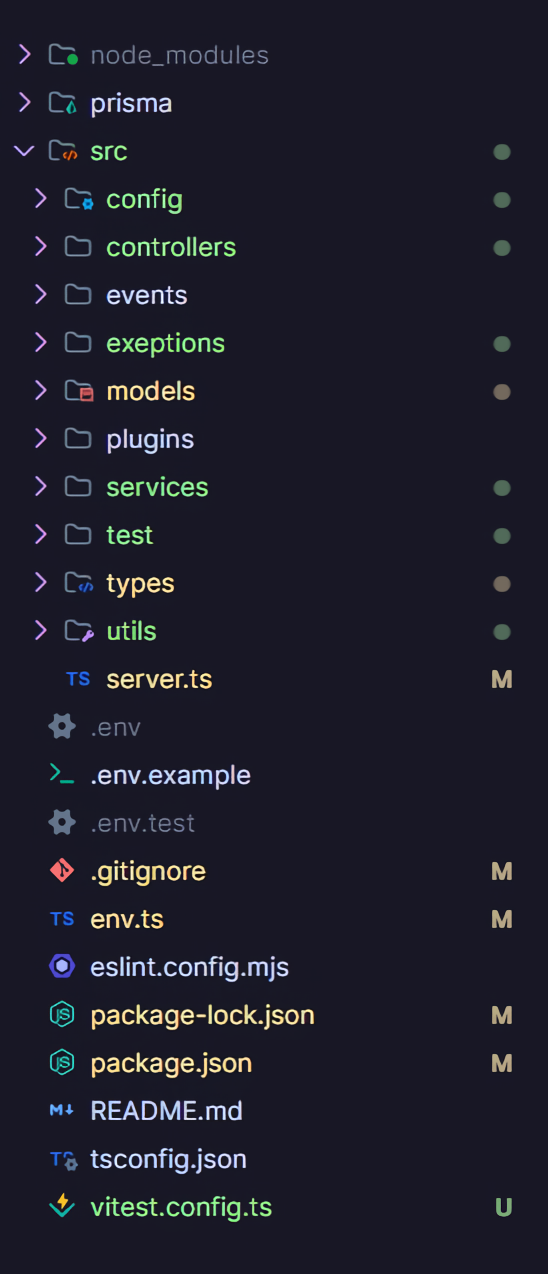
\includegraphics[scale=0.23]{img/pastas.png}
	\legend{Fonte: Autoria Própria}
	\label{fig:EstruturaDePastas}
\end{figure}



% INICIO banco de dados
\subsection{Banco de Dados}

A construção de um banco de dados foi necessário para fazer testes de requisição na \textit{API} desenvolvida. Neste contexto, serão introduzidos o Diagrama Entidade-Relacionamento (DER) e o Modelo Entidade-Relacionamento (MER), para representar graficamente a organização das entidades e os vínculos entre os dados no sistema. Em seguida, serão descritos o esquema do banco de dados, suas tabelas e os relacionamentos estabelecidos entre elas. Essas representações visuais ajudam na compreensão da estrutura lógica e física do banco de dados, bem como facilita o processo de manutenção e expansão futura do software.

\subsection{Diagrama Entidade-Relacionamento (MER)}

A construção deste diagrama conceitual foi de suma importância para a modelagem de dados, representando o mini mundo em questão de um possível aplicativo de caronas. Transformar um recorte do mundo real, para o significado dos dados e como eles se relacionam colaboram na precisão das buscas de informações armazenadas no servidor. O \textit{``Anexo A''} mostra o diagrama entidade-relacionamento deste projeto.


\subsection{Modelo Entidade-Relacionamento (DER)}

Após a modelagem do diagrama anterior, foi possível utilizar o BrModelo para realizar a conversão das tabelas necessárias no banco de dados. O DER facilita a compreensão do MER, tornando a estrutura do banco de dados mais intuitiva e visual, detalhando as chaves primárias, estrangeiras e as cardinalidades. O \textit{``Anexo B''} apresenta as tabelas convertidas, suas chaves e cardinalidades.

\subsection{Dicionário de Dados}

O Dicionário de Dados é uma utilizada em projetos acadêmicos e de desenvolvimento de software, pois descreve detalhadamente as tabelas que compõem o banco de dados relacional, bem como seus atributos. Esta seção tem como objetivo proporcionar uma visão clara e organizada da estrutura do banco de dados, listando as entidades e suas respectivas características. No contexto deste trabalho, as principais tabelas incluem Usuários, Endereços, Motoristas, Veículos, Viagens, Reservas, Mensagens e Avaliações. As tabelas de 1 a 11 apresentam as descrições de cada tabela do banco, incluindo suas principais colunas e uma breve explicação dos atributos mais relevantes.

% tabela de usuário
\begin{longtblr}[
	caption = {Descrição da Entidade Usuários. },
	label = {tab:requisitos},
	entry = none,
	]{
		width = \linewidth,
		colspec = {Q[190]Q[160]Q[620]},
		row{1} = {c},
		row{2} = {c},
		cell{1}{1} = {c=3}{0.938\linewidth},
		cell{3}{1} = {c},
		cell{3}{2} = {c},
		cell{4}{1} = {c},
		cell{4}{2} = {c},
		cell{5}{1} = {c},
		cell{5}{2} = {c},
		cell{6}{1} = {c},
		cell{6}{2} = {c},
		cell{7}{1} = {c},
		cell{7}{2} = {c},
		cell{8}{1} = {c},
		cell{8}{2} = {c},
		cell{9}{1} = {c},
		cell{9}{2} = {c},
		cell{10}{1} = {c},
		cell{10}{2} = {c},
		cell{11}{1} = {c},
		cell{11}{2} = {c},
		cell{12}{1} = {c},
		cell{12}{2} = {c},
		cell{13}{1} = {c},
		cell{13}{2} = {c},
		cell{14}{1} = {c},
		cell{14}{2} = {c},
		cell{15}{1} = {c},
		cell{15}{2} = {c},
		cell{16}{1} = {c},
		cell{16}{2} = {c},
		cell{17}{1} = {c},
		cell{17}{2} = {c},
		hlines,
		vlines,
	}
	\textbf{Usuários}                &                         &                  \\
	\textbf{NOME}                    & \textbf{TIPO DE DADOS}  & \textbf{DESCRIÇÃO}\\
	
	{(PK)\\id\_usuario} 			 & VARCHAR                 & Chave primaria Identificador único da tabela ``usuarios''.\\
	
	nome                             & VARCHAR                 & Nome do usuário.\\
	
	{segundo\_nome}                  & VARCHAR                 & Sobrenome do usuário.\\
	
	email                            & VARCHAR~                & E-mail único, utilizado para login.\\
	
	senha                            & VARCHAR~                & {Senha forte, com no mínimo 8 caracteres, incluindo\\letras maiusculas, minúsculas, números e caracteres\\especiais.} \\
	
	telefone                         & VARCHAR                 & Número de telefone válido.\\
	
	foto\_perfil                     & VARCHAR~                & Caminho para a foto de perfil do usuário.\\
	
	eh\_motorista                    & BOOLEAN                 & Diferencia o usuário do motorista.\\
	
	ativo                            & BOOLEAN                 & Salva a informação se o usuário é ativo.\\
	
	{classificacao\\\_media}         & DOUBLE                  & Nota média do usuário.\\
	
	data\_criacao                    & DATE                    & Armazena a data da criação do perfil.\\
	
	data\_atualizacao                & DATE                    & Ultima atualização do usuário.
	
\end{longtblr}



% Tabela TOKEN
\begin{longtblr}[
	caption = {Descrição da Entidade Token.},
	label = {tab:requisitos},
	entry = none,
	]{
		width = \linewidth,
		colspec = {Q[190]Q[160]Q[620]},
		row{1} = {c},
		row{2} = {c},
		cell{1}{1} = {c=3}{0.938\linewidth},
		cell{3}{1} = {c},
		cell{3}{2} = {c},
		cell{4}{1} = {c},
		cell{4}{2} = {c},
		cell{5}{1} = {c},
		cell{5}{2} = {c},
		cell{6}{1} = {c},
		cell{6}{2} = {c},
		cell{7}{1} = {c},
		cell{7}{2} = {c},
		cell{8}{1} = {c},
		cell{8}{2} = {c},
		hlines,
		vlines,
	}
	
	\textbf{Token}        &                        &                                               \\
	
	\textbf{NOME}         & \textbf{TIPO DE DADOS} &  \textbf{DESCRIÇÃO}\\
	
	{(PK)\\id\_token}	  &     VARCHAR            &  Chave primária, identificador único da tabela ``token''. ~\\
	  
	token      			  &     VARCHAR            &  Armazena o token único gerado para a solicitação de recuperação de senha. \\
	
	{expiracao\_em} 	  &     DATETIME           &  Armazena a data e hora em que o token expira.~\\
	
	{(FK)\_usuarios}	  &     VARCHAR   	       &  Chave estrangeira, referência à tabela ``usuarios''.
	
\end{longtblr}


% Tabela Mensagens
\begin{longtblr}[
	caption = {Descrição da Entidade Mensagens.},
	label = {tab:requisitos},
	entry = none,
	]{
		width = \linewidth,
		colspec = {Q[190]Q[160]Q[620]},
		row{1} = {c},
		row{2} = {c},
		cell{1}{1} = {c=3}{0.941\linewidth},
		cell{3}{1} = {c},
		cell{3}{2} = {c},
		cell{4}{1} = {c},
		cell{4}{2} = {c},
		cell{5}{1} = {c},
		cell{5}{2} = {c},
		hlines,
		vlines,
	}
	\textbf{MENSAGENS}    &                        &                                                \\
	\textbf{NOME}         & \textbf{TIPO DE DADOS} & \textbf{DESCRIÇÃO}                              \\
	
	{(PK) \\id\_mensagem} & VARCHAR                & Chave primária, identificador único da mensagem. \\
	
	conteudo              & VARCHAR                & Armazena o conteúdo das mensagens trocadas.       \\
	
	data\_envio           & DATETIME               & Data do envio da mensagem.~                       \\
	
	{(FK)\_remetente}     & VARCHAR                & Chave estrangeira, referência à tabela ``usuarios'', representando o usuário que enviou a mensagem.~  \\
	
	{(FK)\_viagens}       & VARCHAR                & Chave estrangeira, referência à tabela ``viagens''.~            \\
	
	{(FK)\\\_destinatario}  & VARCHAR              & Chave estrangeira, referência à tabela ``usuarios'', representando o usuário que recebeu a mensagem.~
	                     
\end{longtblr}


% Tabela VIAGENS
\begin{longtblr}[
	caption = {Descrição da Entidade Viagens.},
	label = {tab:requisitos},
	entry = none,
	]{
		width = \linewidth,
		colspec = {Q[190]Q[160]Q[620]},
		row{1} = {c},
		row{2} = {c},
		cell{1}{1} = {c=3}{0.94\linewidth},
		cell{3}{1} = {c},
		cell{3}{2} = {c},
		cell{4}{1} = {c},
		cell{4}{2} = {c},
		cell{5}{1} = {c},
		cell{5}{2} = {c},
		cell{6}{1} = {c},
		cell{6}{2} = {c},
		cell{7}{1} = {c},
		cell{7}{2} = {c},
		cell{8}{1} = {c},
		cell{8}{2} = {c},
		cell{9}{1} = {c},
		cell{9}{2} = {c},
		cell{10}{1} = {c},
		cell{10}{2} = {c},
		cell{11}{1} = {c},
		cell{11}{2} = {c},
		cell{12}{1} = {c},
		cell{12}{2} = {c},
		cell{13}{1} = {c},
		cell{13}{2} = {c},
		cell{14}{1} = {c},
		cell{14}{2} = {c},
		cell{15}{1} = {c},
		cell{15}{2} = {c},
		cell{16}{1} = {c},
		cell{16}{2} = {c},
		cell{17}{1} = {c},
		cell{17}{2} = {c},
		hlines,
		vlines,
	}
	\textbf{VIAGENS}            &                         &                   \\
	\textbf{NOME}               & \textbf{TIPO DE DADOS}  & \textbf{DESCRIÇÃO} \\
	
	{(PK) \\id\_viagem}         & VARCHAR                 & Chave primária, identificador da tabela viagem.\\
	
	status                      & ENUM                    & Armazena os possíveis status da corrida, variando entre agendado, em andamento, concluído ou cancelado.\\
	
	{data\_criacao}             & DATETIME                & Data da criação da corrida.~\\
	
	preco                       & DECIMAL                 & Preço da corrida, quando aplicável a monetização da mesma.\\
	
	{hora\_termino}             & DATETIME                & Registra a hora que a corrida acaba.\\
	
	{preferencias}              & VARCHAR                 & Preferências da corrida definidas pelos participantes antes do seu início.\\
	 
	{data\_atualizacao}         & DATETIME                & Data de atualização mais recente da viagem.\\
	
	{hora\_partida}             & DATETIME                & Define a hora de início de uma viagem.\\
	
	{lugares\\\_disponiveis}    & INT                     & Armazena a quantidade de assentos disponíveis para os passageiros, de acordo com o veículo cadastrado pelo motorista.\\

	{(FK)\_motorista}           & VARCHAR                 & Chave estrangeira, referência à tabela ``motoristas''.\\ 
	
	{(FK)\_endereco\\\_destino} & VARCHAR                 & Chave estrangeira, referência à tabela ``enderecos'', representando o endereço de destino da viagem.\\
	
	{(FK)\_endereco\\\_partida} & VARCHAR                 & Chave estrangeira, referência à tabela ``enderecos'', representando o endereço de partida da viagem.\\
	
	{(FK)\_veiculo}             & VARCHAR                 & Chave estrangeira, referência à tabela ``veiculos''.\\

\end{longtblr}


% Tabela RESERVAS
\begin{longtblr}[
	caption = {Descrição da Entidade Reservas.},
	label = {tab:requisitos},
	entry = none,
	]{
		width = \linewidth,
		colspec = {Q[190]Q[160]Q[620]},
		row{1} = {c},
		row{2} = {c},
		cell{1}{1} = {c=3}{0.938\linewidth},
		cell{3}{1} = {c},
		cell{3}{2} = {c},
		cell{4}{1} = {c},
		cell{4}{2} = {c},
		cell{5}{1} = {c},
		cell{5}{2} = {c},
		cell{6}{1} = {c},
		cell{6}{2} = {c},
		cell{7}{1} = {c},
		cell{7}{2} = {c},
		cell{8}{1} = {c},
		cell{8}{2} = {c},
		hlines,
		vlines,
	}
	\textbf{RESERVAS}      &                        & \\
	\textbf{NOME}          & \textbf{TIPO DE DADOS} & \textbf{DESCRIÇÃO}\\
	
	{(PK)\\id\_reserva}    & VARCHAR                & Chave primária, identificador único da tabela ``reservas''.\\
	
	{data\_criacao}        & DATETIME               & Armazena a data da criação no momento em que a reserva é feita.~\\
	
	{data\_atualizacao}    & DATETIME               & Armazena a data em que a viagem foi atualizada.             \\
	 
	status                 & ENUM                   & Armazena os possíveis status da reserva, variando entre agendado, em andamento, concluído ou cancelado.\\
	
	{status\\\_pagamento}  & ENUM                   & Armazena os possíveis status de pagamento quando aplicável. \\
	
	{(FK)\_passageiro}     & VARCHAR                & Chave estrangeira, referência à tabela ``usuarios'', representando o usuário que solicita a viagem. ~ \\
	
	{(FK)\_viagens}        & VARCHAR                & Chave estrangeira, referência à tabela ``viagens''. \\
	
	
\end{longtblr}

% Tabela AVALIACOES
\begin{longtblr}[
	caption = {Descrição da Entidade Avaliações.},
	label = {tab:requisitos},
	entry = none,
	]{
		width = \linewidth,
		colspec = {Q[190]Q[160]Q[620]},
		row{1} = {c},
		row{2} = {c},
		cell{1}{1} = {c=3}{0.939\linewidth},
		cell{3}{1} = {c},
		cell{3}{2} = {c},
		cell{4}{1} = {c},
		cell{4}{2} = {c},
		cell{5}{1} = {c},
		cell{5}{2} = {c},
		cell{6}{1} = {c},
		cell{6}{2} = {c},
		cell{7}{1} = {c},
		cell{7}{2} = {c},
		cell{8}{1} = {c},
		cell{8}{2} = {c},
		hlines,
		vlines,
	}
	\textbf{AVALIAÇÕES}   &                        &  \\
	\textbf{NOME}         & \textbf{TIPO DE DADOS} & \textbf{DESCRIÇÃO}\\
	
	{(PK)\\id\_avaliacao} & VARCHAR                & Chave primária, identificador único da avaliação.\\
	
	avaliacao             & INT                    & Numeral de 1 a 5 representando a nota da avaliação.\\
	
	comentario            & VARCHAR                & Mensagem de avaliação do usuário.~\\

	{data\_criacao}       & DATETIME               & Data de criação do registro.\\
	
	{data\_atualizacao}   & DATETIME               & Data da modificação mais recente. \\

	{(FK)\_avaliador}     & VARCHAR                & Chave estrangeira, referência à tabela ``usuarios'', representando o usuário que avaliará.   \\
	 
	{(FK)\_viagens}       & VARCHAR                & Chave estrangeira, referência à tabela ``viagens''. \\
	
	{(FK)\_avaliado}      & VARCHAR                & Chave estrangeira, referência à tabela ``usuarios'', representando o usuário que será avaliado.
	
\end{longtblr}


% Tabela ENDEREÇOS
\begin{longtblr}[
	caption = {Descrição da Entidade Endereços.},
	label = {tab:requisitos},
	entry = none,
	]{
		width = \linewidth,
		colspec = {Q[190]Q[160]Q[620]},
		row{1} = {c},
		row{2} = {c},
		cell{1}{1} = {c=3}{0.938\linewidth},
		cell{3}{1} = {c},
		cell{3}{2} = {c},
		cell{4}{1} = {c},
		cell{4}{2} = {c},
		cell{5}{1} = {c},
		cell{5}{2} = {c},
		cell{6}{1} = {c},
		cell{6}{2} = {c},
		cell{7}{1} = {c},
		cell{7}{2} = {c},
		cell{8}{1} = {c},
		cell{8}{2} = {c},
		cell{9}{1} = {c},
		cell{9}{2} = {c},
		hlines,
		vlines,
	}
	\textbf{ENDEREÇOS}        &                        &                           \\
	\textbf{NOME}             & \textbf{TIPO DE DADOS} & \textbf{\textbf{DESCRIÇÃO}}\\
	
	{(PK)\\id\_endereco}      & VARCHAR                & Chave primária, identificador único do endereço.\\
	
	cidade                    & VARCHAR                & Nome da cidade.\\
	
	longitude                 & DOUBLE                 & Coordenada geográfica que especifica a posição norte-sul de uma cidade específica. É de suma importância nas requisições.\\
	
	latitude                  & VARCHAR                & Coordenada geográfica que especifica a posição leste–oeste de uma cidade específica. É de suma importância nas requisições.\\
	
	{endereco\\\_formatado}   & VARCHAR                & Nome formatado do endereço. Importante para a precisão das pesquisas, uma vez que algumas localizações possuem nomes populares, não registrados pelos serviços de geolocalização.\\
	
	ativo                     & BOOLEAN                & Salva a informação se o endereço é ativo.\\
	
	{data\_criacao}           & DATETIME               & Data de criação do registro.\\
	
	{data\_atualizacao}       & DATETIME               & Data da última atualização. \\
	
	{(FK)\_usuarios}          & VARCHAR                & Chave estrangeria, referência a tabela ``usuarios''.
	
\end{longtblr}


% Tabela VEÍCULOS
\begin{longtblr}[
	caption = {Descrição da Entidade Veículos.},
	label = {tab:requisitos},
	entry = none,
	]{
		width = \linewidth,
		colspec = {Q[190]Q[160]Q[620]},
		row{1} = {c},
		row{2} = {c},
		cell{1}{1} = {c=3}{0.941\linewidth},
		cell{3}{1} = {c},
		cell{3}{2} = {c},
		cell{4}{1} = {c},
		cell{4}{2} = {c},
		cell{5}{1} = {c},
		cell{5}{2} = {c},
		cell{6}{1} = {c},
		cell{6}{2} = {c},
		cell{7}{1} = {c},
		cell{7}{2} = {c},
		cell{8}{1} = {c},
		cell{8}{2} = {c},
		cell{9}{1} = {c},
		cell{9}{2} = {c},
		cell{10}{1} = {c},
		cell{10}{2} = {c},
		cell{11}{1} = {c},
		cell{11}{2} = {c},
		cell{12}{1} = {c},
		cell{12}{2} = {c},
		cell{13}{1} = {c},
		cell{13}{2} = {c},
		hlines,
		vlines,
	}
	\textbf{VEÍCULOS}         &                         &                  \\
	\textbf{NOME}             & \textbf{TIPO DE DADOS}  & \textbf{DESCRIÇÃO}\\
	
	{(PK) \\id\_veiculo}      & VARCHAR                 & Chave primária, identificador único do veículo.\\
	
	data\_atualizacao         & DATETIME                & Data da última alteração dos dados do veículo.~\\
	
	cor                       & VARCHAR                 & Cor do veículo.\\
	
	marca                     & VARCHAR                 & Descreve a marca do veículo.\\
	
	data\_criacao             & DATETIME                & Data de cadastro do veículo.\\
	
	ativo                     & BOOLEAN                 & Verifica se o veículo ainda está ativo na aplicação ou não. \\
	
	ano                       & INT                     & Ano de fabricação do veículo.\\
	
	placa                     & VARCHAR                 & Salva o número da placa do veículo após o seu registro.\\ 
	
	capacidade                & INT                     & Quantidade máxima de passageiros que o veículo registrado deve possuir.\\
	
	modelo                    & VARCHAR                 & Descreve o modelo do veículo.~\\
	
	{(FK)\\\_proprietario}    & VARCHAR                 & Chave estrangeira, referência à tabela ``usuarios'', representando o usuário proprietário do veículo.
	
	
\end{longtblr}

%Fim das tabelas 

\subsection{Relacionamentos}

\begin{enumerate}
	
	
	\item \textbf{Usuários - Reservas}
	\begin{itemize}
		\item (1,N): Um usuário pode fazer várias reservas.
		\item (1,1): Cada reserva é feita por um único usuário.
	\end{itemize}
	
	\item \textbf{Usuários - Avaliações}
	\begin{itemize}
		\item (1,N): Um usuário pode fazer várias avaliações.
		\item (1,1): Cada avaliação é feita por um único usuário.
	\end{itemize}	
	
		\item \textbf{Usuários - Mensagens}
	\begin{itemize}
		\item (1,N): Um usuário pode enviar e receber várias mensagens.
		\item (1,1): Cada mensagem tem um remetente e um destinatário únicos, podendo envolver diferentes usuários.
	\end{itemize}
	
		\item \textbf{Usuários - Endereços}
	\begin{itemize}
		\item (1,N): Um usuário pode ter vários endereços.
		\item (1,1): Cada endereço pertence a um único usuário.
	\end{itemize}
	
		\item \textbf{Usuários - Token}
	\begin{itemize}
		\item (1,N): Um usuário pode ter vários TokenJwtExpirado.
		\item (1,1): Cada TokenJwtExpirado pertence a um único usuário.
	\end{itemize}
	
	\item \textbf{Motoristas - Veículos}
	\begin{itemize}
		\item (1,N): Um motorista pode ter vários veículos.
		\item (1,1): Cada veículo está associado a um único motorista
	\end{itemize}
	
	\item \textbf{Motoristas - Viagens}
	\begin{itemize}
		\item (1,N): Um motorista pode criar várias viagens.
		\item (1,1): Cada viagem é conduzida por um único motorista.
	\end{itemize}
	
	\item \textbf{Viagens - Reservas}
	\begin{itemize}
		\item (1,N): Uma viagem pode ter várias reservas.
		\item (1,1): Cada reserva está associada a uma única viagem.
	\end{itemize}
	
	\item \textbf{Viagens - Avaliações}
	\begin{itemize}
		\item (1,N): Uma viagem pode ter várias avaliações.
		\item (1,1): Cada avaliação é feita para uma única viagem.
	\end{itemize}
	
	\item \textbf{Endereço - Viagens}
	\begin{itemize}
		\item (1,1): Uma viagem tem um endereço associado.
		\item (1,N): Cada endereço pode estar associado a várias viagens.
	\end{itemize}
	
	\item \textbf{Mensagens - Viagens}
	\begin{itemize}
		\item (1,N): Uma viagem pode ter várias mensagens associadas.
		\item (1,1): Cada mensagem pode estar se referir a uma única viagem.
	\end{itemize}
	
	\item \textbf{Veículo - Viagens}
	\begin{itemize}
		\item (1,N): Um veículo pode ser utilizado em várias viagens.
		\item (1,1): Cada viagem utiliza um único veículo.
	\end{itemize}
\end{enumerate}

\section{Front-end}

O desenvolvimento do front-end do aplicativo VemComigo foi orientado para proporcionar uma experiência intuitiva e acessível aos usuários. As escolhas durante esta etapa seguem os conhecimentos adquiridos nas aulas de Banco de Dados II, Análise e Projeto de Sistemas, Práticas Profissionais Integradoras II e Desenvolvimento Web II.

\subsection{Arquitetura do Front-End}

Primeiramente, foi realizada a prototipação das possíveis telas com o auxílio de um projeto criado no Figma, o qual pode ser acessado por meio do link:[https://abrir.link/PMhoA]. Criou-se pastas no projeto com a finalidade de melhor organizar as projeções do visual da aplicação. Os primeiros esboços visuais da aplicação encontram-se na página ``Wireframes''. O desing de alta fidelidade foi projetado na sequência e pode ser encontrado na página ``Desing'' do projeto. Por fim, para integrar a API do back-end desenvolvida anteriormente ao front-end, escolheu-se o React Native como framework do JavaScript, visando a criação de uma aplicação multiplataforma eficiente e de forma paralela para Android e IOS. Foi necessário utilizar o Expo como uma ferramenta auxiliar nos testes das telas desenvolvidas, garantindo que os componentes estivessem bem posicionados na tela.

\subsection{Design e UX (Experiência do Usuário)}

A interface foi projetada com foco na responsividade, usabilidade e experiência do usuário, permitindo que esses, mesmo que em diferentes dispositivos móveis, tenham uma utilização intuitiva e fluida. O VemComigo é uma aplicação voltada para a mobilidade e deslocamento de pessoas, dito isso, imagina-se que o usuário final busca simplicidade para escolher rapidamente um meio viável de transporte em meio a agitação do dia a dia. Nesse contexto, decidiu-se então que as telas deveriam ser minimalistas de forma que apenas informações necessárias ocupassem espaço na tela, evitando confusões em usuários mais desatentos. A ``tabela \ref{tab:design-ux}'' apresenta as escolhas que compõem o padrão visual da aplicação.

\begin{longtblr}[
	caption = {Design e UX (Experiência do Usuário)},
	label = {tab:design-ux},
	entry = none,
	]{
		width = \linewidth,
		colspec = {Q[170,c]Q[620]},
		row{1} = {c},
		row{2} = {c},
		cell{1}{1} = {c=2}{0.941\linewidth},
		cell{3}{1} = {c},
		cell{3}{2} = {c},
		cell{4}{1} = {c},
		cell{4}{2} = {c},
		cell{5}{1} = {c},
		cell{5}{2} = {c},
		cell{6}{1} = {c},
		cell{6}{2} = {c},
		cell{7}{1} = {c},
		cell{7}{2} = {c},
		hlines,
		vlines,
	}
	\textbf{Design e UX (Experiência do Usuário)} &  \\
	
	\textbf{Aspecto} & \textbf{Descrição} \\
	
	\textbf{Tipografia} & A fonte escolhida para o aplicativo foi a Poppins, uma tipografia moderna e elegante, amplamente utilizada em interfaces digitais por sua excelente legibilidade em diferentes tamanhos de tela. O uso de diferentes pesos (light, regular, semibold e bold) permitiu hierarquizar informações e destacar conteúdos importantes sem comprometer a estética da interface. \\
	
	\textbf{Paleta de Cores} & Cor principal: \#0064D2 (Azul vibrante) – representa confiança, tecnologia e mobilidade.  
	Cor de Fundo: \#FFFFFF (Branco) – proporciona um ambiente limpo e moderno, facilitando a leitura e destacando os elementos interativos. Cores secundárias e de apoio: tons de cinza e azul escuro foram utilizados para equilibrar a interface e manter um visual neutro e sofisticado. \\
	
	\textbf{Componentes Visuais} & A biblioteca de componentes ``Tamagui'' foi utilizada para melhorar os aspectos visuais e garantir a otimização da aplicação. Adotou-se também uma biblioteca de ícones chamada ``Tabler'', disponível em [https://tabler.io/admin-template]. \\
	
	\textbf{Inputs e Formulários} & Os campos de entrada (inputs) foram projetados para serem acessíveis e de fácil identificação. Foram aplicados bordas arredondadas, espaçamento adequado e feedback visual para indicar erros ou sucessos nas interações dos usuários. Os botões seguem um estilo minimalista, utilizando o azul primário (\#0064D2) para submeter ações principais. \\
	
	\textbf{Logo e Identidade Visual} & O logotipo do aplicativo foi desenvolvido para refletir o conceito de transporte de maneira abstrata. Utilizou-se uma abordagem minimalista, incorporando elementos gráficos que remetem a um formato de uma roda. \\
	
	\textbf{Acessibilidade} & Foram aplicadas boas práticas de acessibilidade, garantindo contraste adequado, tamanhos de fonte ajustáveis e navegação intuitiva para todos os usuários. \\
\end{longtblr}


\subsection{Componentização}

A adoção da componentização no desenvolvimento do front-end do aplicativo permitiu a criação de uma interface modular, escalável e de fácil manutenção. Utilizando React Native com o auxílio do Tamagui, os componentes foram desenvolvidos de forma reutilizável, garantindo maior consistência visual e reduzindo a duplicação de código. Entre os principais benefícios dessa abordagem observa-se:

\begin{enumerate}
	\item \textbf{Reutilização de Código:} Componentes como botões e inputs foram desenvolvidos para permitir a sua aplicação em diferentes telas sem necessidade de reescrita.
	\item \textbf{Facilidade de Manutenção:} Alterações no design ou comportamento podem ser feitas em um único local, refletindo automaticamente em todas as instâncias do componente.
	\item \textbf{Melhoria na Performance:} O uso de componentes otimizados reduz a renderização desnecessária, tornando a aplicação mais eficiente.
\end{enumerate}

\subsection{Diagrama de Classes}

O diagrama de classes do VemComigo foi gerado com base no schema do Prisma, refletindo a estrutura dos dados e os relacionamentos entre as entidades da aplicação. Como o projeto utiliza um back-end baseado em Node.js e Prisma ORM, sem a implementação direta de classes, o diagrama representa apenas os modelos de dados, sem a definição de métodos. Entre as principais entidades do sistema, destacam-se Usuário, Veículo, Corrida, Reserva, Endereço e Avaliação, além das tabelas auxiliares como Token e Mensagem. As relações foram modeladas para garantir um fluxo eficiente entre motoristas e passageiros, possibilitando funcionalidades como gerenciamento de corridas, envio de mensagens e sistema de avaliação. Essa estrutura permite a manipulação otimizada dos dados, garantindo escalabilidade e performance na aplicação. O ``Anexo C'' apresenta uma representação gráfica do diagrama de classes.

\subsection{Diagrama de Caso de Uso}

O diagrama de caso de uso do VemComigo representa as interações entre os principais atores do sistema: Passageiro, Motorista e Administrador. Ele ilustra os serviços disponíveis para cada perfil de usuário, destacando funcionalidades como criação de conta, solicitação e gerenciamento de corridas, troca de mensagens entre usuários e sistema de avaliações.  O ``Anexo D'' apresenta uma representação gráfica do diagrama de classes. Em síntese, a ``Tabela \ref{tab:atores-casosdeuso}'' descreve os atores da aplicação e algumas das suas principais ações no sistema.

\begin{longtblr}[
	caption = {Atores e Casos de Uso do Aplicativo},
	label = {tab:atores-casosdeuso},
	entry = none,
	]{
		width = \linewidth,
		colspec = {Q[250,c]Q[650,l]},
		row{1} = {c},
		hlines,
		vlines,
	}
	\textbf{Ator} & \textbf{Casos de Uso} \\
	
	\textbf{Passageiro} & 
	Criar conta, Fazer login, Solicitar uma carona, Cancelar reserva, Ver histórico de corridas, Avaliar motorista, Gerenciar endereço salvo, Enviar mensagem ao motorista. \\
	
	\textbf{Motorista} & 
	Criar conta, Fazer login, Cadastrar veículo, Criar corrida, Cancelar corrida, Gerenciar reservas recebidas, Ver histórico de corridas, Avaliar passageiro, Enviar mensagem ao passageiro. \\
	
	\textbf{Administrador} & 
	Gerenciar usuários, Gerenciar corridas, Monitorar avaliações. \\
	
\end{longtblr}



\section{Tecnologias e Ferramentas}

O desenvolvimento de software exige uma variedade de recursos durante a produção. Escolher cuidadosamente as ferramentas a serem utilizadas no ambiente de desenvolvimento garante a qualidade, funcionalidade, eficácia, escalabilidade e eficiência do sistema. Nesse contexto, as tecnologias empregadas durante o desenvolvimento do trabalho serão descritas a seguir. 

\subsection{Ambiente de Trabalho}

\begin{enumerate}
	\item\textit{Visual Studio Code} - editor de código-fonte gratuito que permite a integração com \textit{Git}, facilitando \textit{commits, pushes, pulls e merges}, além de possibilitar o uso do \textit{intelliSense} para melhorar a produtividade no ambiente de trabalho.
	
	\item \textit{GitHub} -  plataforma de hospedagem de código-fonte que permite o versionamento \textit{Git}. Foi importante para que cada colaborador trabalhasse na implementação das mudanças nos repositórios da organização.
	
	\item \textit{Node.js} -  Ferramenta de execução e interpretação da linguagem \textit{JavaScript} que permite o seu uso no ambiente de desenvolvimento, sendo utilizado para executar os códigos criados ao lado do servidor com tal linguagem. 
\end{enumerate}


\subsection{Linguagem de Programação}

\begin{enumerate}
	\item \textit{JavaScript} -   linguagem de programação escolhida devido a sua  versatilidade, facilidade de uso, sintaxe limpa e grande oferta de \textit{frameworks.}
	\item \textit{TypeScript} - é o superset do \textit{JavaScript} que adiciona tipagem estática à linguagem,  permitindo com que o desenvolvedor possa definir os tipos de dados das suas variáveis, funções e objetos com a finalidade de tornar o código mais seguro, previsível e escalável, além de facilitar futuras refatorações.

\end{enumerate}

\subsection{\textit{Framework}}

\begin{enumerate}
	\item\textit{Fastify} - Uma das melhores opções entre os frameworks para \textit{Node.js,} sendo rápido, flexível e com uma excelente experiência de desenvolvimento. Foi utilizado para construir aplicações web escaláveis e de alto desempenho, além de oferecer uma boa integração com o \textit{TypeScript.} 
\end{enumerate}

\subsection{Banco de Dados}

\begin{enumerate}

	\item \textit{Prisma - Object-Relational Mapper (ORM)} escolhido para as interações com o banco de dados, sendo necessário para criar migrações, assim criar, ler, atualizar e deletar dados no banco de dados se tornou mais rápido e com menos código, reduzindo a possibilidade de erros.
	
	\item \textit{MySQL} - Sistema Gerenciador de Banco de Dados (SGBD) responsável por armazenar, organizar e gerenciar dados. É conhecido pela confiabilidade e ampla utilização nos mais variados ambientes de desenvolvimento.
	
	\item BrModelo -  foi uma ferramenta importante na modelagem do banco de dados, permitindo a elaboração de diagramas entidade-relacionamento (ER) e facilitando a sua visualização antes da implementação da versão final do banco.
	
\end{enumerate}

\subsection{Produtividade}

\begin{enumerate}
	
	\item \textit{Trello} - Utilizado para o gerenciamento do projetos baseado em metodologia visual, por meio de um sistema de quadro de \textit{Kanban}, dividindo uma tarefa em várias ações para que todos os integrantes do grupo participem do projeto de forma coesa.
	
	\item \textit{Notion} -  Necessário para os desenvolvedores centralizarem as informações importantes, bem como anotações desenvolvidas ao longo do trabalho. Entre as suas vantagens destaca-se a facilidade de uso e a integração com outras ferramentas.
	
\end{enumerate}



% ---
% Conclusão
% ---
\chapter{CONSIDERAÇÕES FINAIS}
% ---

A mobilidade entre as cidades do Vale do Jequitinhonha, especialmente no contexto do atual ciclo de extração de lítio, apresenta desafios significativos devido à escassez de veículos e à oferta limitada de serviços de transporte. A análise da frota de veículos e a comparação com o tamanho da população evidenciam a necessidade de soluções práticas para facilitar o deslocamento entre os municípios.

Além disso, a desigualdade na oferta de serviços em cada cidade intensifica as migrações pendulares, o que sobrecarrega as opções de transporte disponíveis atualmente. Nesse cenário, a implementação de um aplicativo de caronas pode ser uma solução inovadora, capaz de formalizar uma prática já existente, porém de forma mais segura e eficiente. Tal proposta visa não apenas garantir maior acessibilidade ao transporte, mas também promover preços justos e aumentar a oferta de viagens, contribuindo para o desenvolvimento socioeconômico da região.

Durante o desenvolvimento do \textit{back-end} foi possível criar vários \textit{endpoints} importantes para garantir um funcionamento inicial adequado, o que facilitou integrações com o \textit{frontend} futuramente. 

Poderão ser implementadas novas funcionalidades no \textit{back-end}, como integração com serviços de pagamento e validação de documentos. O projeto será desenvolvido com foco em escalabilidade, segurança de dados e alta disponibilidade, assegurando uma experiência fluida e segura tanto para motoristas quanto para passageiros.

As funcionalidades de criação de conta, cadastro de motorista, autenticação de usuário e reserva de carona estão plenamente funcionais, além de seguirem o conceito do \textit{Create, Read, Update, Delete (CRUD)}, essencial na criação de sistemas. 

A escolha do \textit{React Native} para o \textit{front-end} possibilitou a criação de uma versão inicial de aplicativo mobile multiplataforma com uma interface intuitiva e estável. Elementos visuais foram escolhidos visando a usabilidade e acessibilidade do projeto, criando uma identidade visual bem definida que busca a melhor experiência de uso, seja para passageiro ou motorista.

Por fim, a nova estruturação do projeto buscou a integração bem definida entre o \textit{front-end} e \textit{back-end}, permitiu uma demonstração mais clara do escopo do projeto. Com isso, espera-se que o aplicativo atenda às necessidades dos usuários e ofereça uma opção de serviço eficiente e seguro, promovendo um modelo de mobilidade compartilhada acessível e sustentável na região.



% ----------------------------------------------------------
% ELEMENTOS PÓS-TEXTUAIS
% ----------------------------------------------------------
\postextual

% ----------------------------------------------------------
% Referências bibliográficas
% ----------------------------------------------------------
\bibliography{referencias}


% ----------------------------------------------------------
% Anexos
% ----------------------------------------------------------

% ---
% Inicia os anexos
% ---
\begin{anexosenv}


\begin{landscape}

	% ---
	\chapter{MODELO ENTIDADE-RELACIONAMENTO (MER)}
	% ---
	
	\begin{figure}[htb!]
		\centering
		\caption{Modelo Conceitual - Aplicativo de Caronas.}
		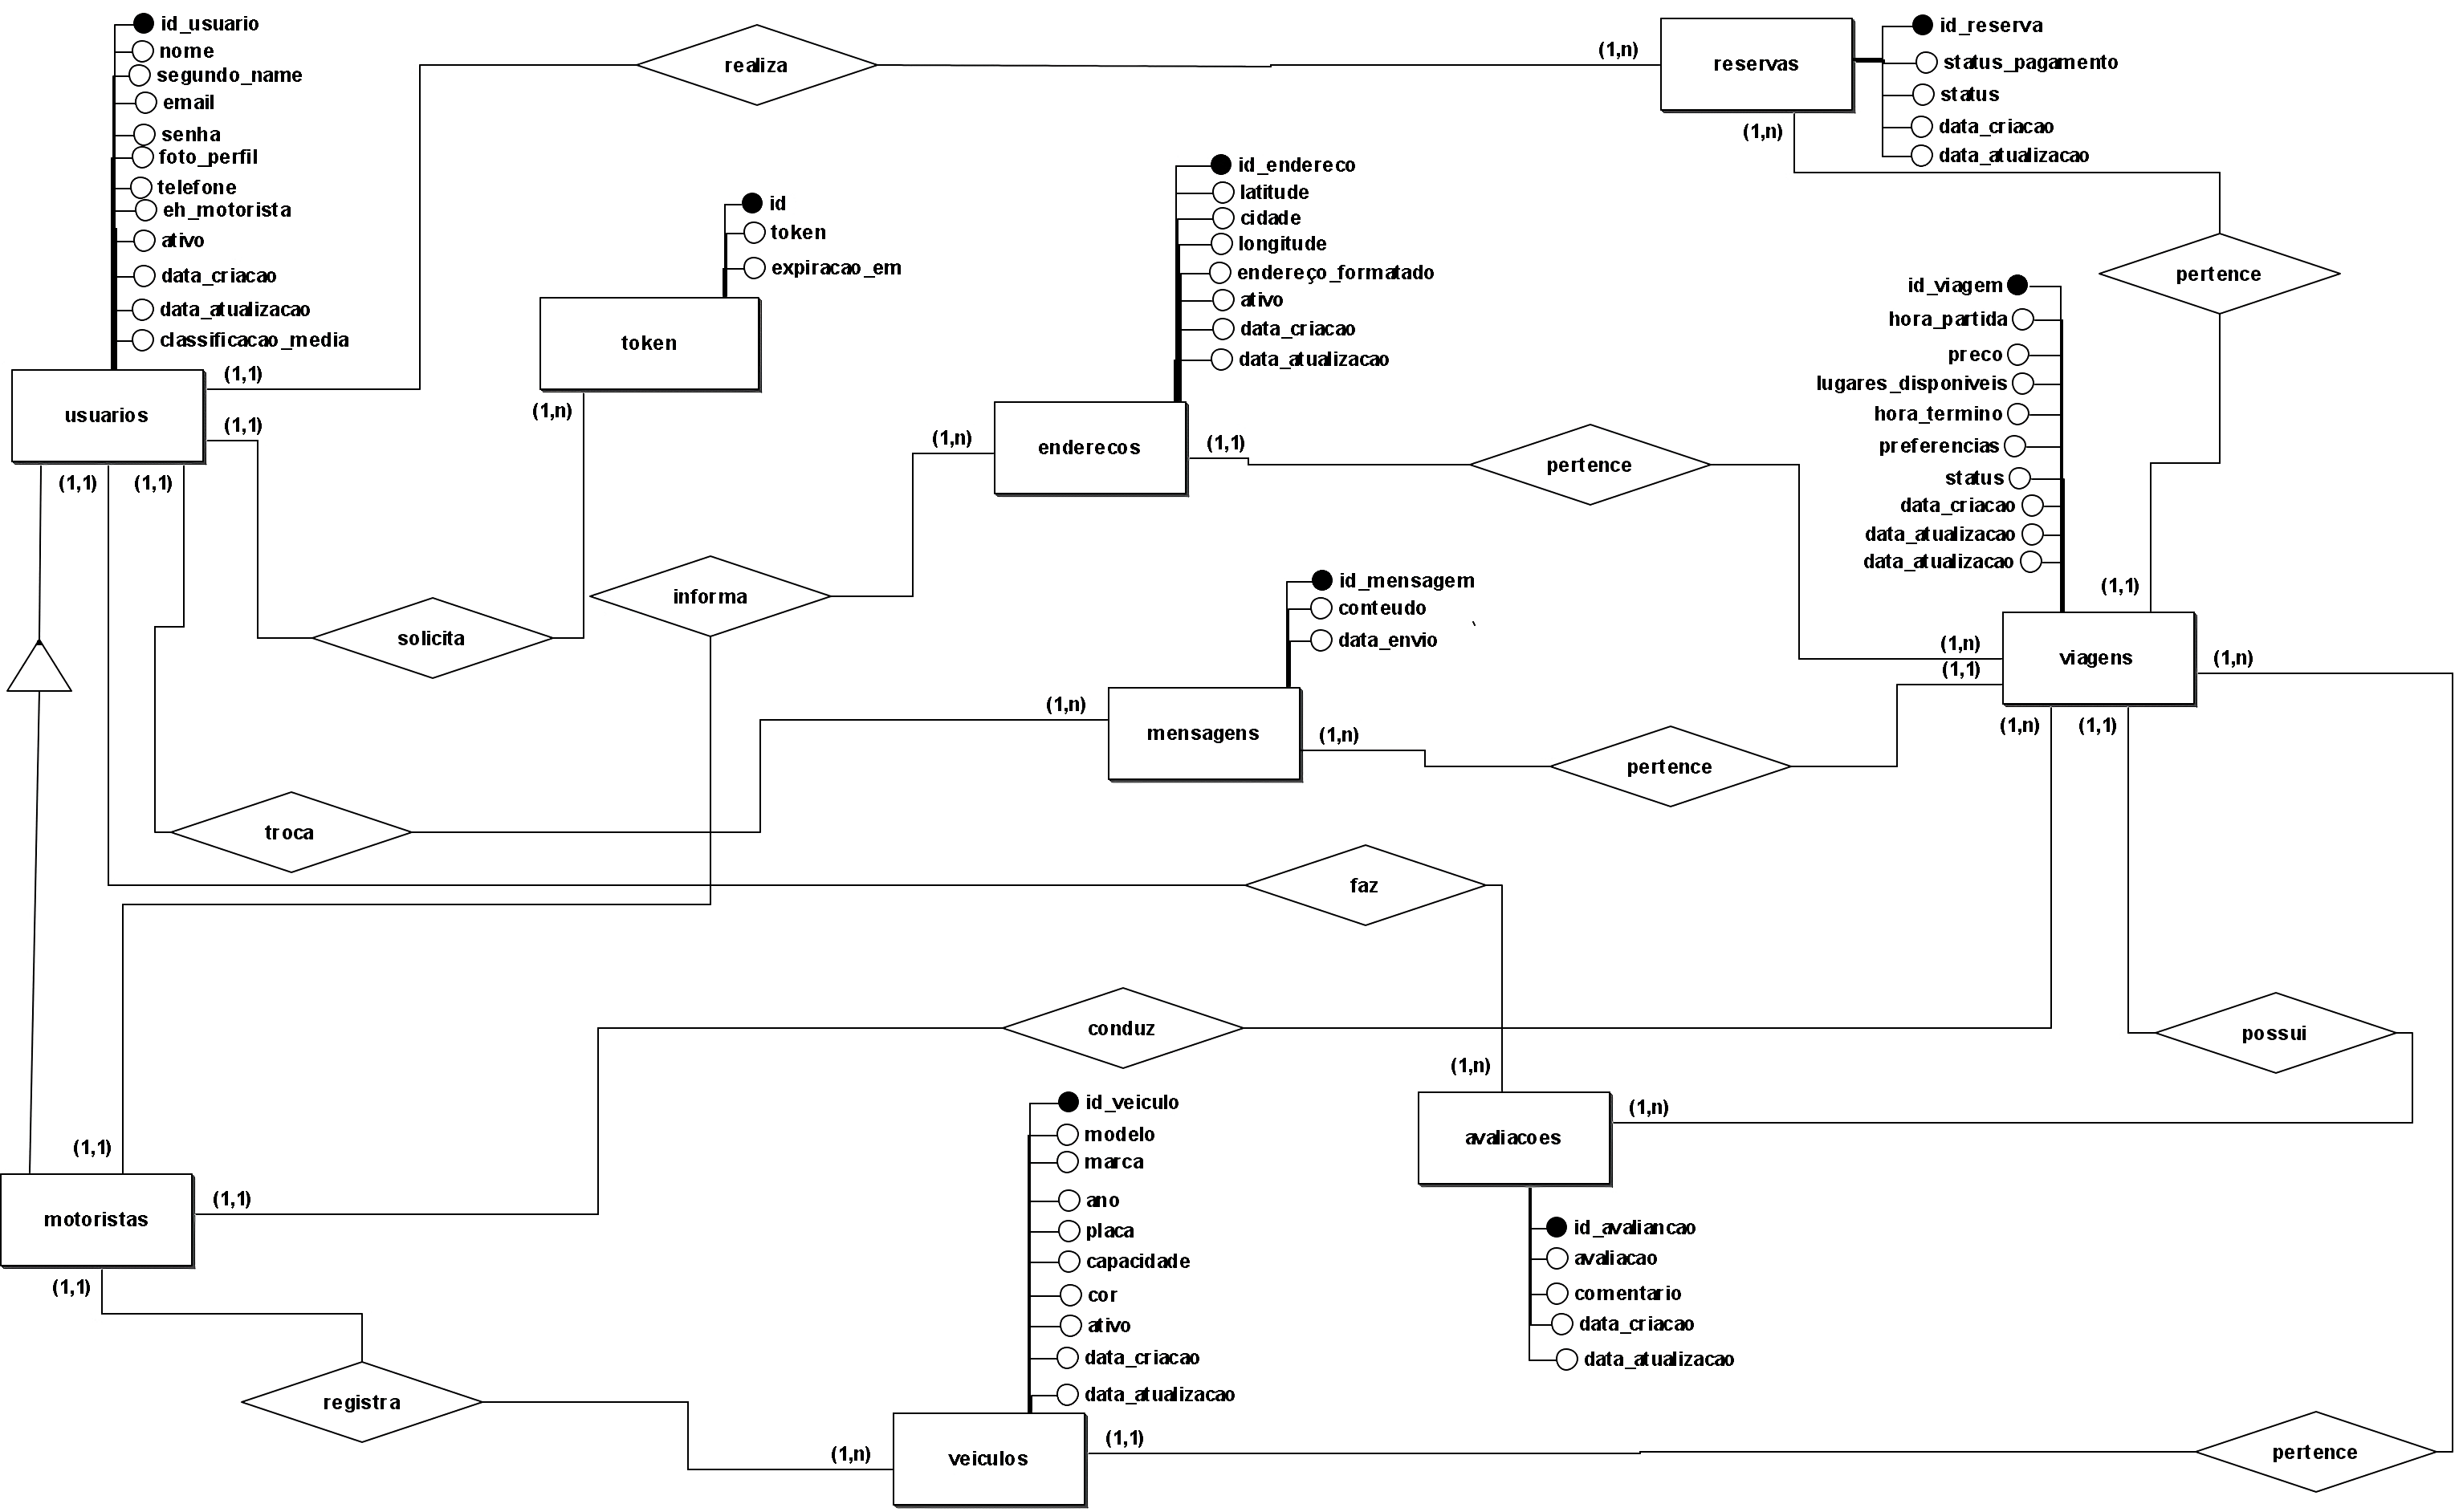
\includegraphics[width=1.45\textwidth]{img/ModeloConceitualIntegradoredit.png} 
		\legend{Fonte: Autoria Própria}
		\label{fig:modelo_conceitual_banco}
	\end{figure}
	
\end{landscape}


\begin{landscape}
	
	% ---
	\chapter{DIAGRAMA ENTIDADE-RELACIONAMENTO (DER)}
	% ---
	
	\begin{figure}[htb!]
		\centering
		\caption{Modelo Lógico - Aplicativo de Caronas.}
		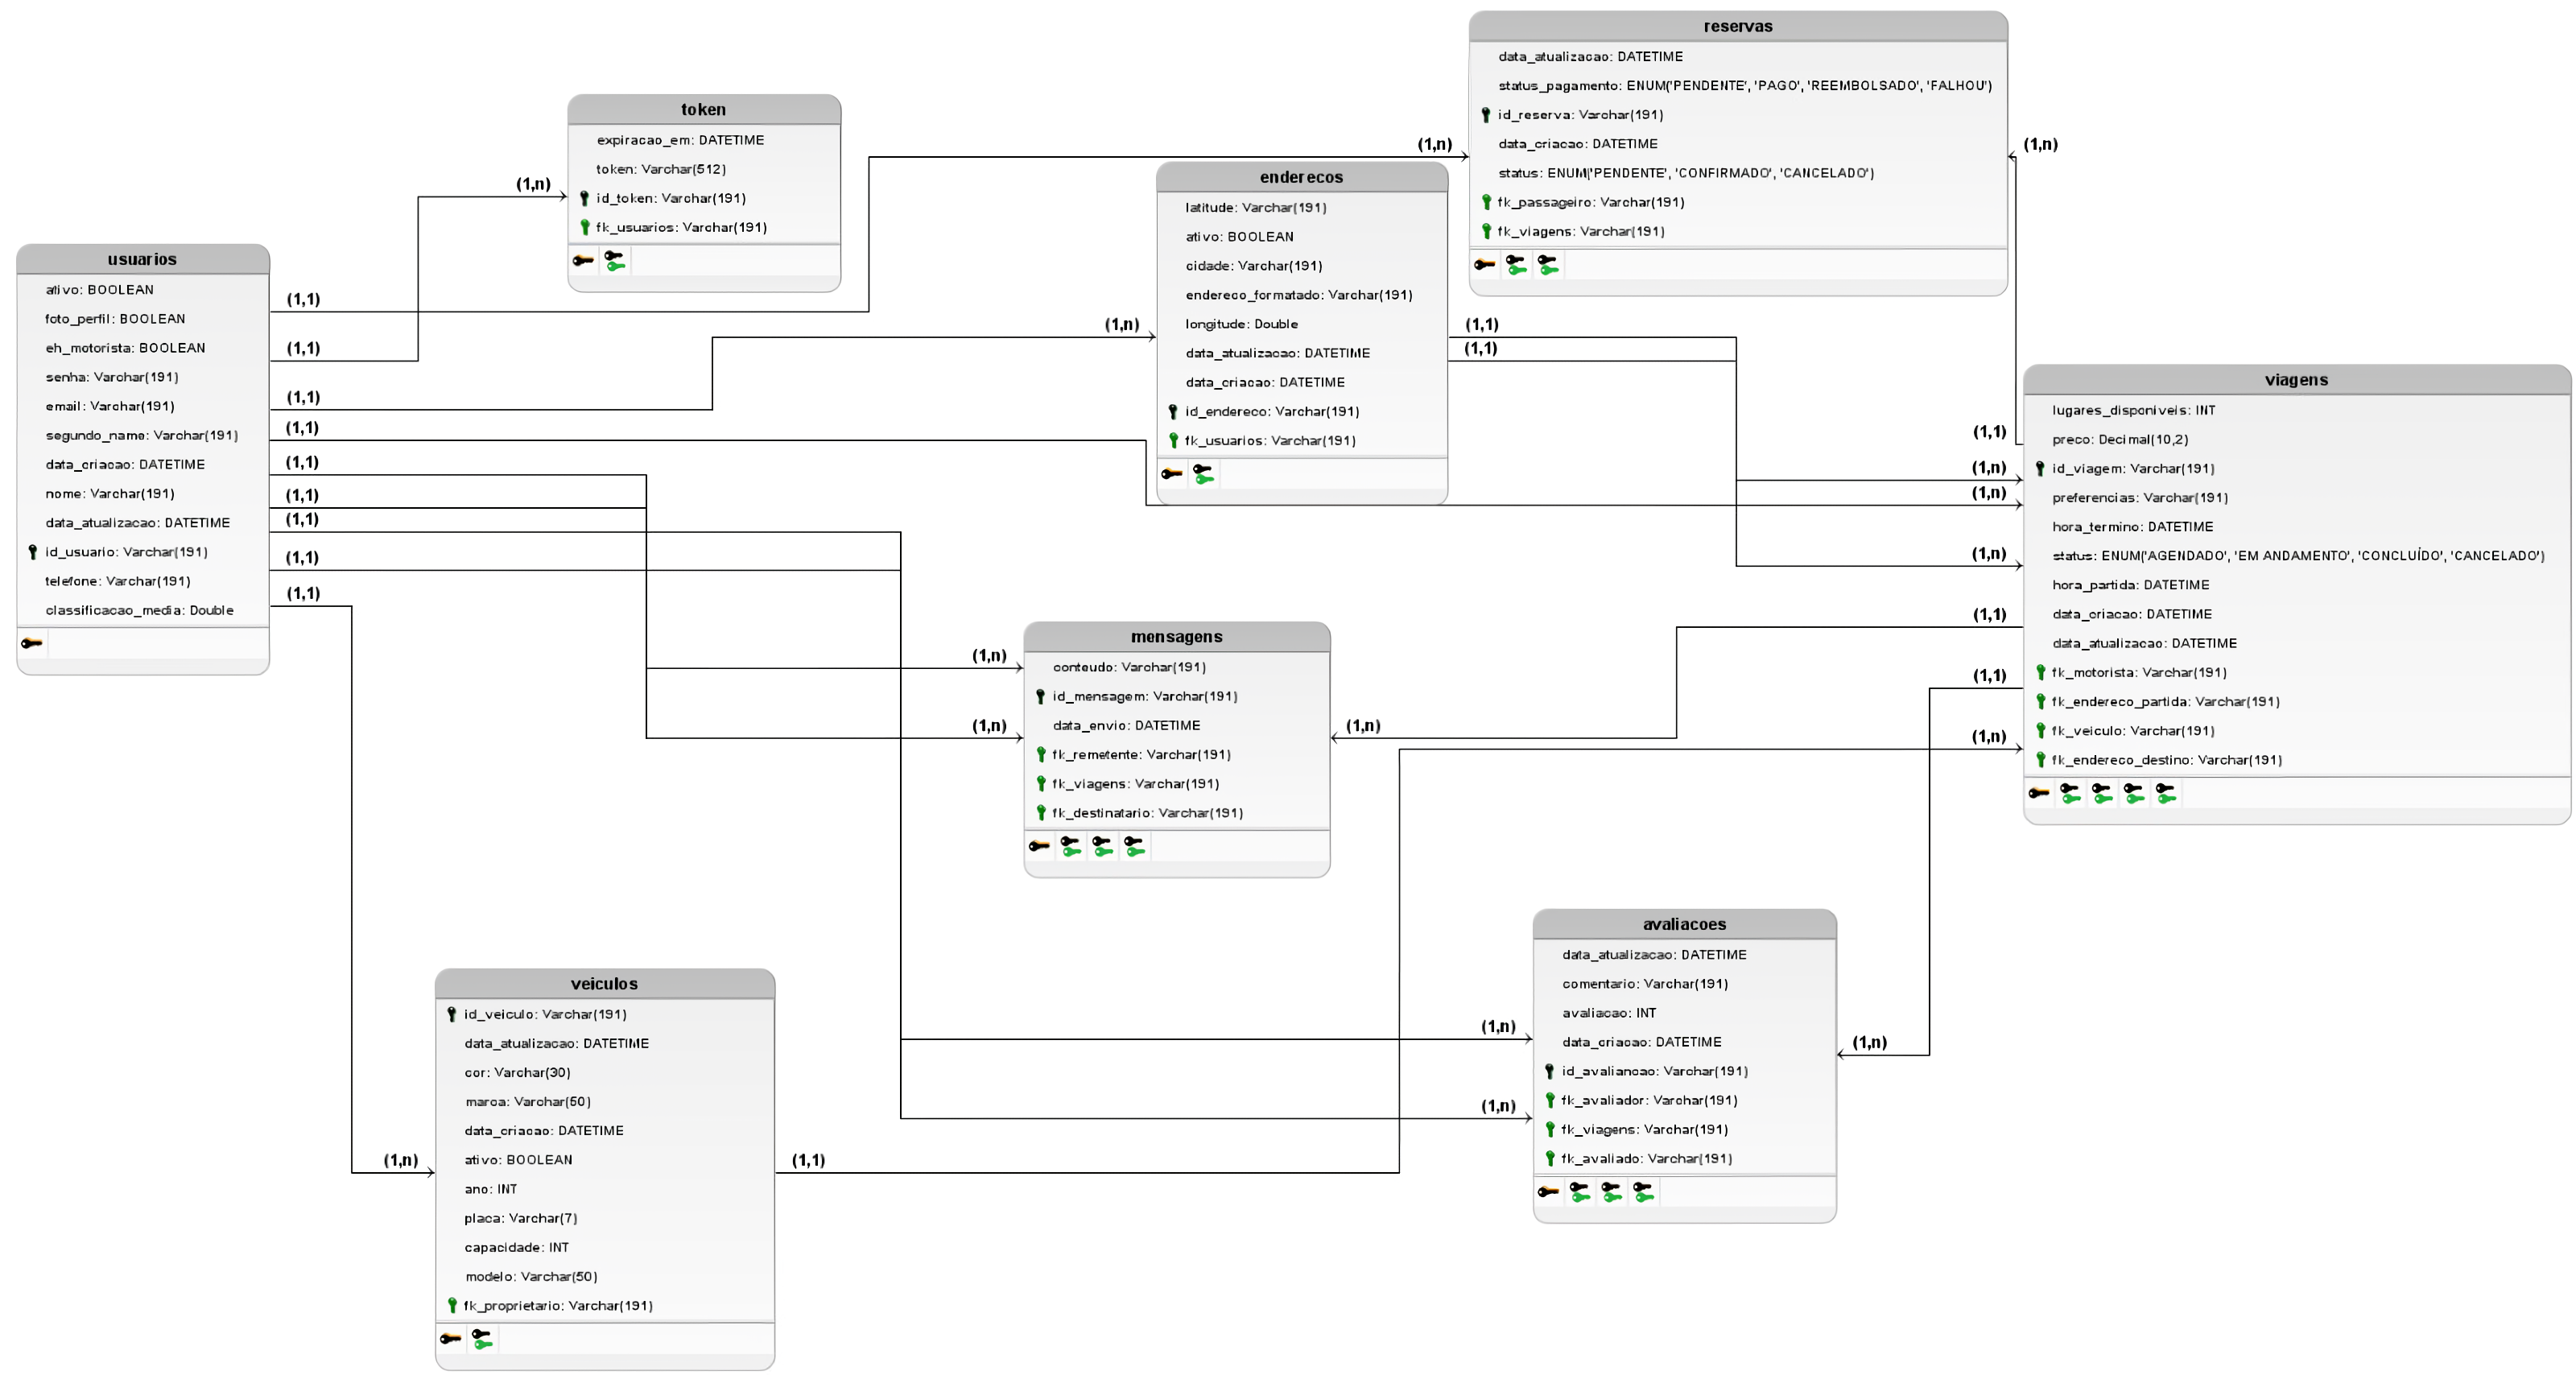
\includegraphics[width=1.45\textwidth]{img/ModeloLogicoIntegradoredit.png}
		\legend{Fonte: Autoria Própria}
		\label{fig:modelo_logico_banco}
	\end{figure}
	
\end{landscape}

\begin{landscape}
	
	% ---
	\chapter{DIAGRAMA DE CLASSES}
	% ---
	
	\begin{figure}[htb!]
		\centering
		\caption{Diagrama de Classes - VemComigo.}
		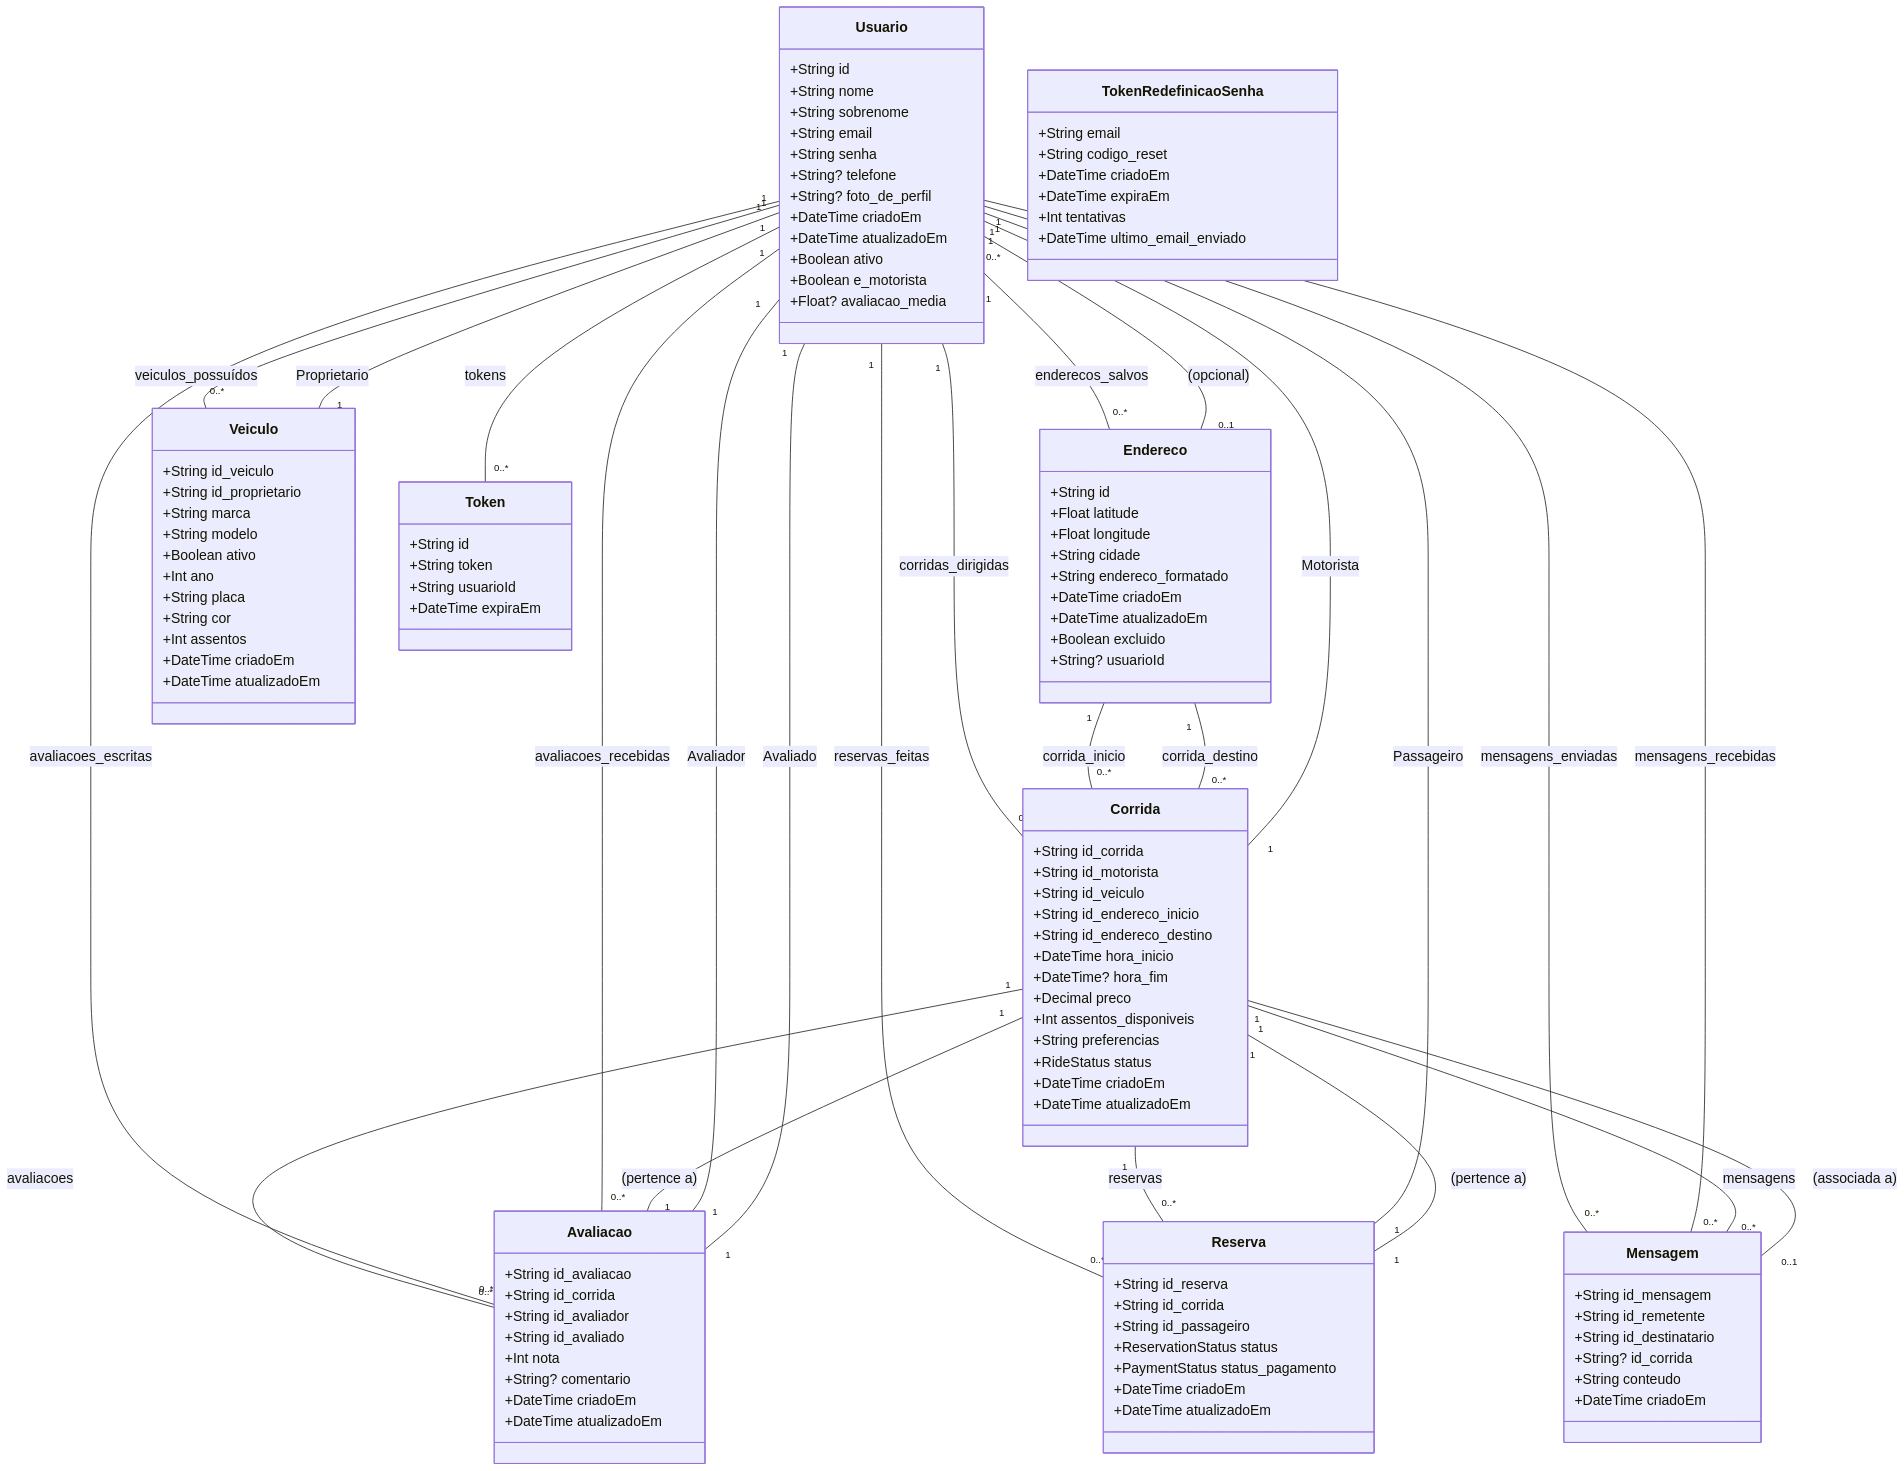
\includegraphics[width=1.25\textwidth]{img/diagrama_classes.png}
		\legend{Fonte: Autoria Própria}
		\label{fig:diagrama_classes}

	\end{figure}
	
\end{landscape}

	
% ---
\chapter{DIAGRAMA DE CASO DE USO}
% ---

\begin{figure}[htb!]
	\centering
	\caption{Diagrama de Caso de Uso - VemComigo.}
	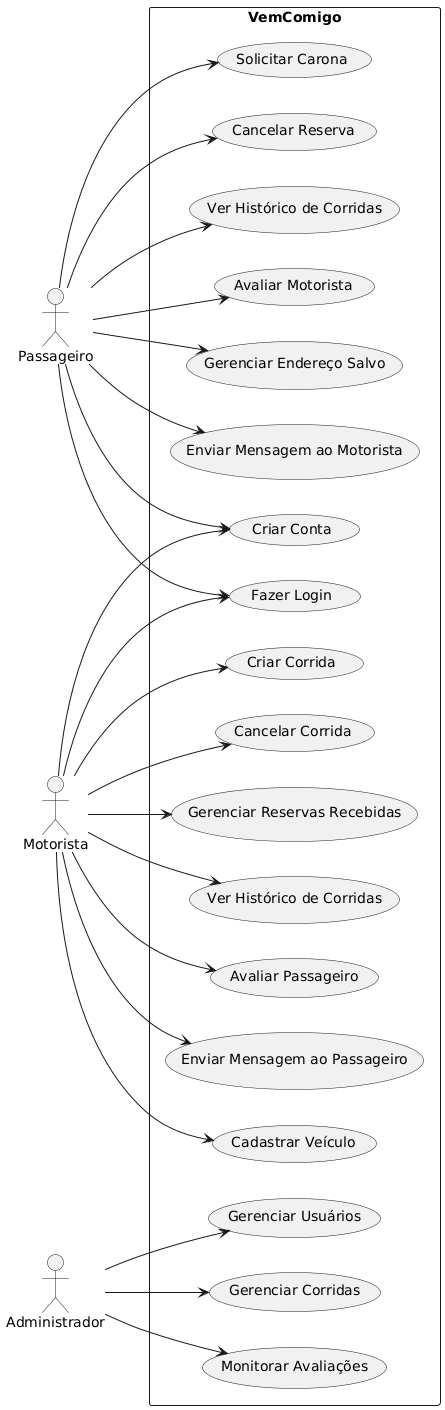
\includegraphics[width=0.47\textwidth]{img/diagrama_caso.png}
	\legend{Fonte: Autoria Própria}
	\label{fig:diagrama_caso}
\end{figure}

\end{anexosenv}


\printindex

%----
% Define tabela 

%----

\end{document}
